%!TEX root = main.tex
\chapter{Filters}
\label{chap:filters}


\begin{figure}[H]
	\begin{center}
		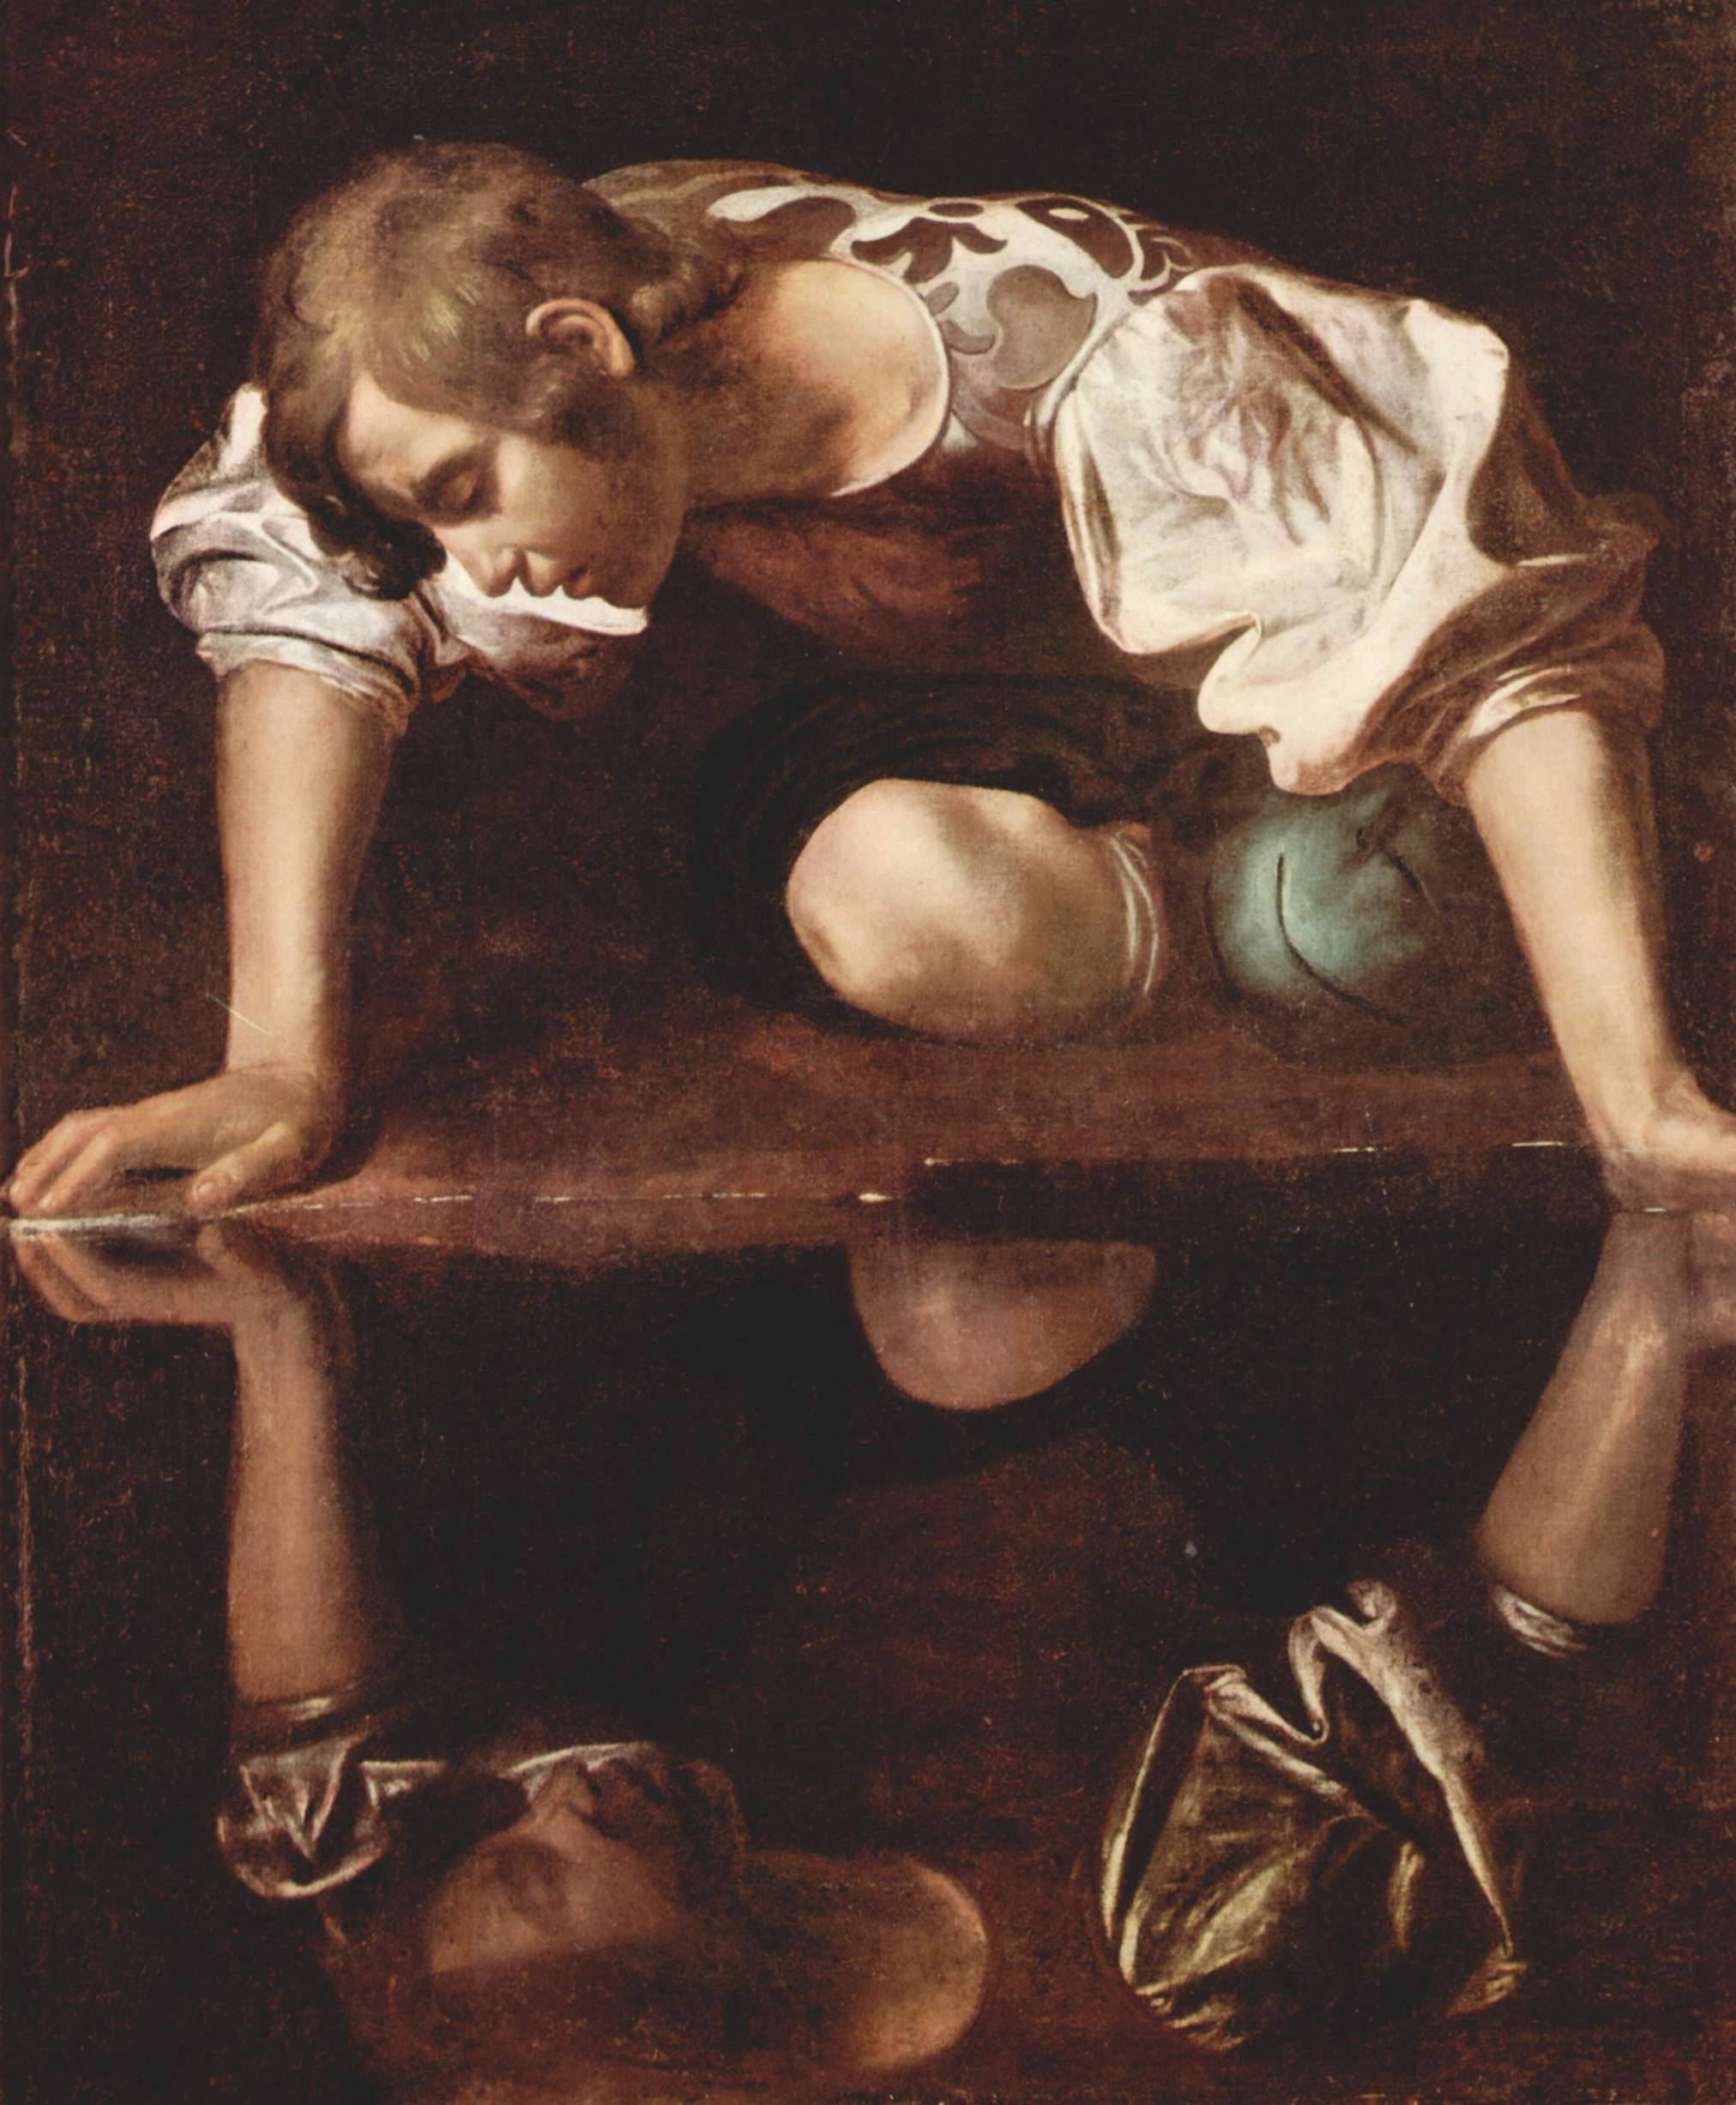
\includegraphics[width = 14cm]{img/Narciss_Caravaggio.jpg}
		\caption{Caravaggio, Narziss. ad Feedback: Echo liebt Narziss etc.}
		\label{fig:name}
	\end{center}
\end{figure}



\comm{lecture mind map missing}


What is a filter? We use filters a lot. We often need to shape the spectrum of a signal. Be it for technical reasons (DC-Offset removal, Anti-aliasing filters, crossovers, interpolation, ...) or for aesthetic ones (EQ-ing, subtractive synthesis)\\
Please take a moment and seriously ask yourself, knowing what you know about signals, knowing what we can do with a computer: How do we actually do this? What is a digital Filter? This is what this chapter will try to explain.\\

\section{Seeing Frequency Content in the Time Domain}

Let's first try to get a fell for how signals \textit{look}. It's a lot easier to understand how a filter works afterwards. This might be obvious but let's state clearly:

\begin{framed}
	High frequency signals have a short \textit{period}. That means the signal ``moves'' fast, or a lot in short time. Therefore: The more movement is in a signal or the more fluctuation or the faster the signal changes the more high frequency content it has.
\end{framed}


Three Questions in order to make you think about signals:


\begin{question}
	Please look at the image below. Can you draw an approximation of its spectrum? What signals could have been mixed to obtain this result?
% subsection raetsel (end)
\begin{figure}[H]
	\begin{center}
		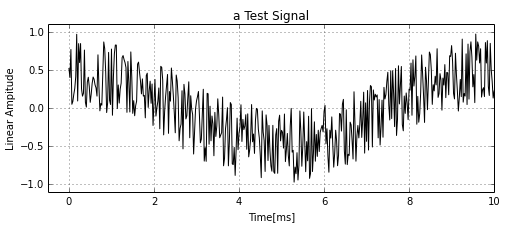
\includegraphics[width = 14cm]{raetsel_original.png}
		\caption{Original Signal}
		\label{fig:originalSignal}
	\end{center}
\end{figure}
\end{question}


\begin{Answer}
You should be able to see that there is a sinusoidal component in the signal. This sinusoid has a period of 10 ms, so a frequency of 100 Hz. But also you should see that it is not a clean sine wave, there is some noisy component in there. This is what you should have been able to infer from the image. In fact it is an (attenuated) 100Hz sinusoid mixed with (attenuated) white noise.
\end{Answer}


\begin{question}
	The signal in figure \ref{fig:originalSignal} was filtered. As a result we obtained the signal in figure \ref{fig:filtered1}. What kind of filter could have been used?
	\begin{figure}[H]
	\begin{center}
		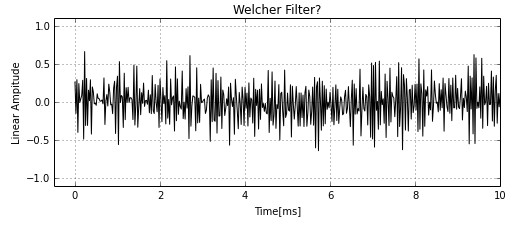
\includegraphics[width = 14cm]{raetsel_highpass.png}
		\caption{Filtered Signal 1}
		\label{fig:filtered1}
	\end{center}
	\end{figure}
\end{question}

\begin{Answer}
	It could have been a notch or stopband filter at 100 Hz or a highpass. In fact, it was a highpass.
\end{Answer}


\begin{question}
	Again, the signal in figure \ref{fig:originalSignal} (so the original signal again) was filtered. As a result we obtained the signal in figure \ref{fig:raetsel_2} . What kind of filter could have been used?
\begin{figure}[H]
	\begin{center}
		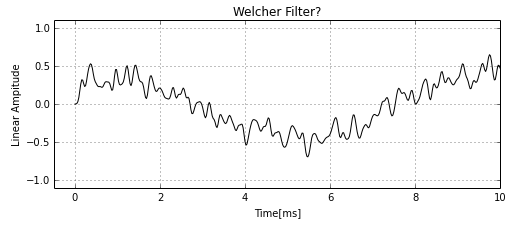
\includegraphics[width = 14cm]{raetsel_lowpass.png}
		\caption{Filtered Signal 2}
		\label{fig:raetsel_2}
	\end{center}
\end{figure}

\end{question}


\begin{Answer}
	It could have been a bandpass at 100Hz, or a lowpass. In fact, it was a lowpass. We see that the signal got a lot smoother.
\end{Answer}

\section{Ways of Describing a Filter}
There are a couple of ways to \textit{fully} describe a linear time invariant system (LTI), filters typically\footnote{filters can be augmented with non-linear or time-varying elements, for example distortion or modulation. In sound design, this is actually very common. But describing such a system mathematically is out of the scope of this work.} are such systems.\\
Below is an (incomplete) list of methods that are all able to describe a filter. They offer very different possibilities of understanding and manipulating a filter.
\begin{itemize}
	\item Difference Equation
	\item Magnitude and Phase Response
	\item Impulse Response
	\item Code (graphical, such as pd)
	\item Code (text, such as C++)
	\item Block Diagram
	\item Transfer Function (Rational Function)
	\item Unit Step Response
\end{itemize}

While in practice, the transfer function is very important, we will mostly work with block diagrams, pd programs and difference equations.\\
It is an important skill to be able to switch between these representations, for example to calculate the impulse response from a difference equation or block diagram.

\subsection{Difference Equations}
\label{sub:diff}

A difference equation is of the form mentioned in the introduction. So for example 
\begin{equation}
	y(n) = x(n)+x(n-1)
	\label{eq:simple}
\end{equation}
Here, $y$ is the output $x$ is the input and $n$ denotes indexing those two signals.\\
$y(n)=x(n)$ means: take the incoming sample and make it the output. $x(n-1)$ denotes a delay by one sample. Please note that the above equation describes a \textit{system}, a filter in this case. But it can be seen as using an input array (the input signal), indexed by $n$ and creating an output array.\\
Let's visualize this idea. Given the input signal in figure \ref{fig:diffImpResp}, we can create the output using the equation. Also it becomes obvious that the $n-1$ expression is a delay, since it makes us look up the 3rd index for creating the 4th sample at the output in this case, or $y(4) = x(4)+x(4-1)$.
\begin{figure}[h!]
	\centering
	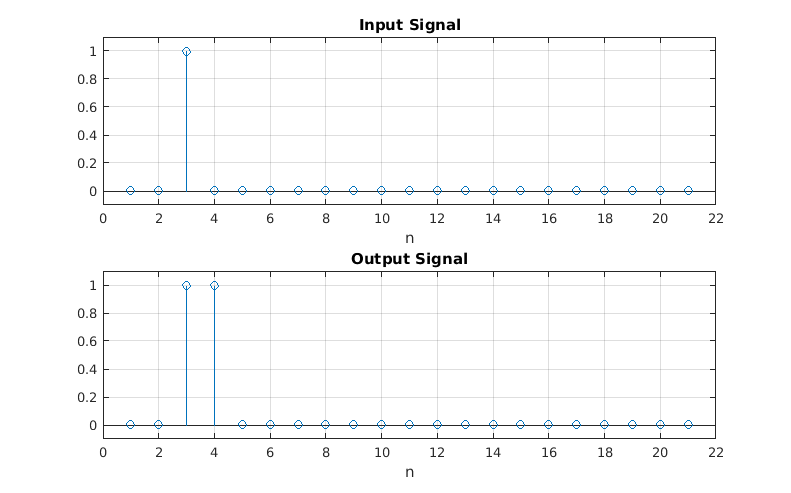
\includegraphics[width=\textwidth]{diffEqViz1}
	\caption[shortCaption]
	{The input and corresponding output of the equation given above.}
	\label{fig:diffImpResp}
\end{figure}


\subsection{Block Diagrams} % (fold)
\label{sub:block}

Block diagrams are nice because they are very visual and sometimes easier to understand. Also, if we work in pure data, or a different graphical programming language (such as Max/MSP or MAYTLAB Simulink) it's very straight forward to implement a block diagram. Translating from a block diagram to text code or difference equations or vice versa can be hard sometimes.\\
In figure \ref{fig:diffImpResp}, we can see a block diagram representation of equation \ref{eq:simple}. This \textit{is} the same thing. 

% subsection subsection_name (end)

\begin{figure}[H]
  \centering  
  \label{fig:string}
  \begin{tikzpicture}[auto, thick, node distance=2.5cm, >=triangle 45]
  \draw node at (0,0) [input] (inp) {};
  \draw node at (2.5,-0.001) (junct) {\textbullet};
  \draw node at (4,2) [block] (delay) {\Large$z^{-1}$};
  \draw node [sum, right of=inp, node distance = 5.cm] (sum1) {\Large$+$};
  
  \draw node [output, right of=sum1,node distance = 3cm] (out) {};
  \draw[->] (inp) -- node {}(sum1);
  % \draw[->] (junct) |- node {}(delay);
  \draw[->] (delay.east) -| node {}(sum1.north);

  \draw[->] (2.5, -0.001) |- node {}(delay.west);


  \draw[->] (sum1) -- node {\Large$y[n]$}(out);
    
  \node[text width=3cm] at (1.7,0.4) 
    {\Large$x[n]$};

  \end{tikzpicture}
  \caption{A very simple lowpass filter.}
  \label{fig:blockDiagr}
\end{figure}

Don't be irritated by the $z^{-1}$ block. This notation stands for a delay by one sample. A block $z^{-m}$ would stand for a delay by $m$ samples. This is a convention we need to remember. This way of notating a delay might seem unnecessarily complex, but it has its reasons.

\bgInfo{This notation, $z^{-1}$, comes from the fact that analyzing the frequency response of a system is very easy when working with complex numbers (so compounds of real and imaginary numbers). Complex numbers are often denoted by $Z$, which is another convention. Not only do we work with complex numbers, but with complex sinusoids when analyzing such systems. We imagine complex sinusoids coming into our system. A multiplication by another complex sinusoid can cause a phase shift (a delay). And this multiplication}


\subsection{pd Code} % (fold)
\label{sub:pd_code}
If we program the filter in pd (or any other programming language) we obviously also fully defined the filter. Try to build the filter from above in pd! Start from the difference equation or the block diagram, what ever is harder to understand for you.\\
In figure \ref{fig:pdSimpleFir} you can see the translation to pd.

\begin{figure}[H]
	\centering
	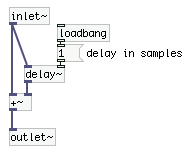
\includegraphics[width=5cm]{simpleFir}
	\caption[FIR filter in pd]
	{A simple filter in pure data.}
	\label{fig:pdSimpleFir}
\end{figure}

% subsection pd_code (end)

\subsection{Impulse Response}

In impulse has the advantage that it contains all frequencies. It has a flat spectrum.  So recording how a filter reacts to the impulse gives us the magnitude of the spectrum at all frequencies.\\
We can see the impulse response of the filter we are describing in this section in  multiple ways in figure \ref{fig:diffImpResp}.

\bgInfo{
\subsection{Text Oriented Code} % (fold)
\label{sub:tcode}
Below, we can see a code implementation in the language MATLAB.

\lstinputlisting[label=code,
captionpos=b,
caption=A script that creates an impulse implements a vectorized filter and plots the result.]{code/FIRvectorized.m}

}
% FIRvectorized.m


% subsection code (end)

% \begin{figure}[htb]
%   \centering  
%   \label{fig:string}

%   \begin{tikzpicture}[auto, thick, node distance=2.3cm, >=triangle 45]

%   \draw node at (0,0) [input] (excitation) {};
%   \draw node [sum, right of=excitation, node distance = 2.cm] (sum1) {\Large$+$};
%   \draw node [block, right of=sum1, node distance = 2cm] (delay) {\Large$z^{-m}$};
%   \draw node [block, below of=delay, node distance = 2cm] (loss) {\Large$G(z)$};
%   \draw node at (6.,-0.001) {\textbullet};

%   \draw node [output, right of=delay,node distance = 3cm] (out) {};
%   \draw[->] (excitation) -- node {\Large$x[n]$}(sum1);
%   \draw[->] (sum1) -- node {}(delay);
%   \draw[->] (loss.west) -| node {}(sum1.south);

%   \draw[->] (6., -0.001) |- node {}(loss.east);


%   \draw[->] (delay) -- node {\Large$y[n]$}(out);
    
%   \end{tikzpicture}
%   \caption{einzelne Saite, $G(z)$ ein lowpass, \glqq{}Loss Filter\grqq{}}
% \end{figure}


\section{Two Ways of Getting an Intuitive Understanding}

So now we learned some ways to define a filter, to talk about a filter. But what is this filter actually doing? It is a very simple lowpass filter. It cuts away high frequencies. But why is adding a signal to itself but one sample delayed making a lowpass? This certainly is a bit surprising, so let's try to understand what's happening.

\subsection{Combfilter to Lowpass}
First let's view the problem from another angle. We know what this structure from above is: It's a combfilter, right? It's taking a signal and adding a delayed version of it. Let's quickly review what a combfilter is:
The combfilter effect can come up if we record something with a microphone and we get the direct signal and a delayed (e.g. via a reflection) signal also. These two signals mix together and this is what we get in our recording.\\
The result is that some frequencies cancel out.\\
We can simply simulate this situation in pd using a delay and an addition. 

\begin{figure}[H]
	\centering
	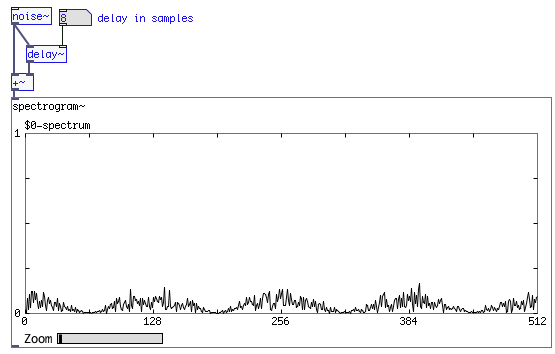
\includegraphics[width=11cm]{simpleComb}
	\caption[shortCaption]
	{realCaption}
	\label{fig:label}
\end{figure}

This canceling out of frequencies \footnote{also called destructive interference} can be imagined if we look at figure \ref{fig:destIntereference}. 
\begin{figure}[H]
	\centering
	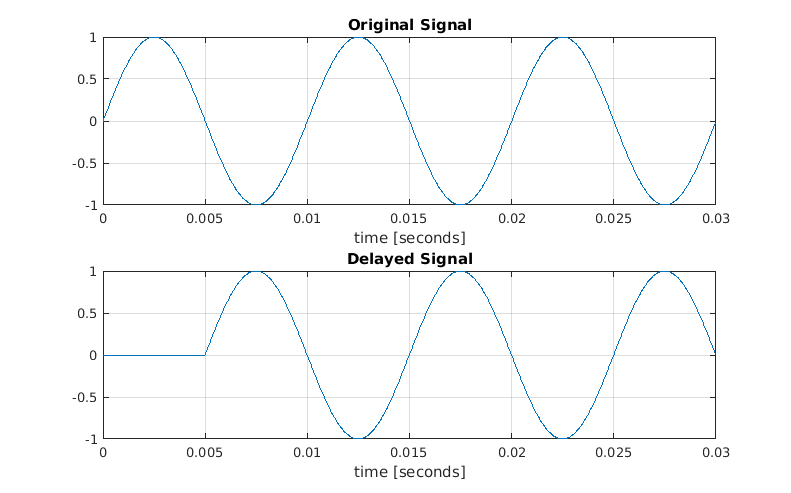
\includegraphics[width=\textwidth]{destInterference}
	\caption[Destructive Interference]
	{Destructive Interference. The two waves would cancel out completely if mixed together(=added).}
	\label{fig:destIntereference}
\end{figure}

Please note that the signal is a sine wave with a frequency of 100 Hz, so a period of 10 milliseconds. The delay is set to be 5 ms, so half of the period of the input signal in this case. It it was set to be equals the period, the two waves would \textit{interfere constructively}, so we would get out a higher amplitude. \\

\important{In a combfilter, the first frequency that cancels out is the one whose period is double the delay time. Or, to put it differently
\begin{equation}
	f_c = \frac{1}{2d}
\end{equation}
If $f_c$ is the first frequency that cancels out and d is the delay time in seconds.

}

In figure \ref{fig:combToLowpass} we can see the \textit{frequency response}\footnote{The impulse response is recorded a couple of times and the output's spectrum has been analyzed} of our combfilter. We see a couple of plots, it's always the same filter but the delay is different. We see that for delay times >1 sample, we observe our typical comb pattern. But at Delay = 1 sample, there is just a ramp left, leaving us with a lowpass.

\begin{figure}[H]
	\centering
	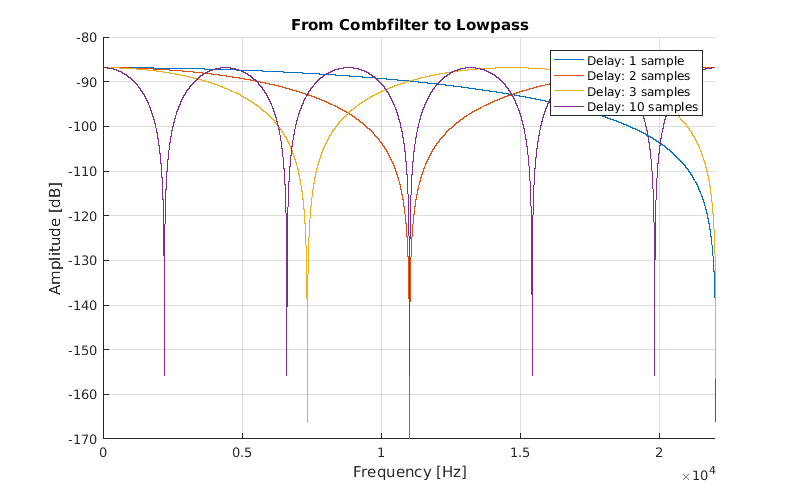
\includegraphics[width=\textwidth]{FromCombfilterToLowpass}
	\caption[shortCaption]
	{realCaption}
	\label{fig:combToLowpass}
\end{figure}

\bgInfo{
	We can also calculate what's happening with our equation from above:
	The delay is $1/f_s$, so 1 over samplerate. This is called the sampling intervall, let's call it $I_s$, just to get rid of the fraction. The frequency that cancels out is then $1/2I$. By inspection we find that this means the frequency that has double the wavelength of the sampling frequency, so half the sampling frequency, so \textit{Nyquist}. 
}


\subsection{Prolonging an Impulse}
We can also take a different route to understand why this is a lowpass. Let's recall what the spectrum of an impulse looks and what the spectrum of DC offset looks like.
\comm{missing figure}






% Notizen aus erster UE:\\
% Viellt. mit IR anfangen?
% Vielleicht davor noch: das beispiel mit noise + sinus.

% IR, bypass system, hall system.

% garnicht faltung. Moving average zu long FIR.
% Impuls antworten anhand beispielen besprechen.


% \begin{enumerate}
% 	\item FIR!

% kammfilter(FF)

% dann FIR kammfilter

% chorus
% flanger

% LFO

% ->index/tiefe, offset, frequenz wdh.


% -frequenzgang
% ausl\"oschungen, rechnen..

% \item 
% FIR one sample delay\\

% FIR bauen, vllt. an tafel blockdiagramm.\\

% FIR hipass\\


% \item 

% mehrere Samples delay
% IR
% differenzen gleichung

% eventuell Faltung(faltungs hall connection herstellen)

% faltung als multiplikation d. spektra
% multiplikation als faltung d spektra.

% M4L faltungs hall herzeigen

% LTI?

% differentiator, akkumulator?

% \item
% IIR\\



% notizen POlyphonie
% was separat, was einmal

% \end{enumerate}

% \section{einfuehrung} % (fold)
% \label{sub:einfuehrung}


% Ziel der LV:\\
% \begin{enumerate}
% 	\item Gefühl dafür bekommen was die häufigsten Operationen der DSV eigentlich tun.
% 	\item Gefühl dafür bekommen, dass es günstig ist, zwischen verschiedenen repräsentationen hin und her zu wechseln (time und frequency domain, aber auch system repräsentationen)
% 	\item Sich in professioneller literatur(DSP lehrbücher) nicht völlig verloren fühlen.
% 	\item schönheit zu sehen dass alles das \glqq{}gleiche\grqq{} ist.(Delay, filter, reverb, chorus, flanger etc)
% \end{enumerate}

% Wozu?:\\
% \begin{enumerate}
% 	\item Wir arbeiten ständig mit Operationen der DSV. Filter sind nicht nur in synthesizern. Ein tieferes verständnis erleichtert die arbeit. Wie funktioniert zum beispiel ein blur?
% 	\item Was ist ein FeedForward compressor?
% \end{enumerate}


% Nachdenken über filter allgemein. Was ist ein filter im gespür d. studenten. \\
% Bekannt was ein LTI system ist?\\


% \newpage
% -Wie könnte ein filter realisiert werden?\\
% -Ein digitales signal ist eine reihe von zahlen, eine sequenz von werten. (über bildliche darstellungen sprechen)\\
% -Echtzeit fall: ich bekomme in ein system ein signal(also ständig werte) und soll ein zb. lowpass gefilteretes signal ausgeben.\\
% \textbf{Was kann ich mit dem signal machen? Zum beispiel addieren, multiplizieren, verzögern.}\\


% Einfacher moving average. Zunächst nur an der tafel!
% Impulsantowrt ausrechnen!
% Was ist ein impuls.\\
% Was ist eine impulsantwort? Beispiele.. untit impulse ( = dirac impuls, dirac gunktion, delta function)\\

% Diagramm aufmalen:

% impuls \(\rightarrow\) Raum \(\rightarrow\) Impulsantwort\\
% oderr \\
% impuls \(\rightarrow\) beliebiges system \(\rightarrow\) Impulsantwort\\
% \textbf{anwendugsbeispiel:} tontechnik bei okto; mischpult ausmessen, dbmax ausmessen(fragwürdige sache! Wieso?)




% \textbf{FRAGE}\\
% Ein system(zB. ein Filter) hat folgende Eigenschft:\\
% Wenn zwei signale getrennt (d.h. unabhängig voneinander, zB. nacheinander.) in das system geschickt werden, und die Ergebnisse summiert werden, entsteht das signal \(P\). Wenn andererseits die signale zuvor summiert werden und dann in das system geschickt werden entsteht ebenfalls \(P\). Welche gleichung etspricht einer beschreibung dieser eigenschaft?



% \begin{enumerate}
% 	\item \(f(x)+f(y) = f (x * y) = P\)
% 	\item \(f(x)+f(y) = f (x + y) = P\)
% 	\item \(f(x)+f(x) = f (x + y) = P\)
% 	\item \(f(x)+f(y) = f (x + x) = P\)
% 	\item nichts von alledem.
% \end{enumerate}

% \newpage
% richtig : nr.2 \\
% \\

% Erklärung eines LTI systems:

% \begin{itemize}
% 	\item Linear:
% 		\begin{itemize}
% 			\item Superpositionsprinzip \(f(x)+f(y) = f (x + y)\)
% 			\item Homogenität \(a*f(x) = f(a*x)\) 
% 		\end{itemize}
% 	\item Time Invariant (zeit-invariant)
% \end{itemize}


% Zurück zu filter: 
% was glauben sie wie er funktioniert. \\
% \\

% \section {kammfilter}

% Wiederum fragen was sich die studenten vorstellen.\\


% \glqq{}Wir bauen ein delay.\grqq{}
% nicht vergessen: block~, subpatcher.


% \begin{figure}[h]
% 	\begin{center}
% 		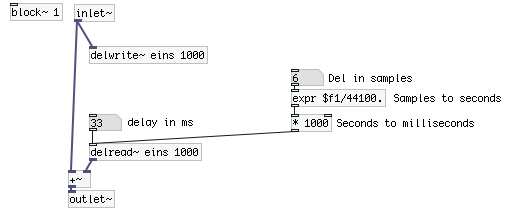
\includegraphics[width = 14cm]{simpleDelay.png}
% 		\caption{SimpleDelay}
% 		\label{fig:simpleDelay}
% 	\end{center}
% \end{figure}

% Studenten sollen ausprobieren. Verschiedene inputs f. kammfilter. \\

% Modulation des kammfilters. Studenten sollen LFO an den kammfilter dran bauen.\\
% \(\rightarrow\) Flager \\
% \(\rightarrow\) Chorus \\

% \textbf{index/tiefe, offset, frequenz wiederholen.}


% \begin{figure}[h]
% 	\begin{center}
% 		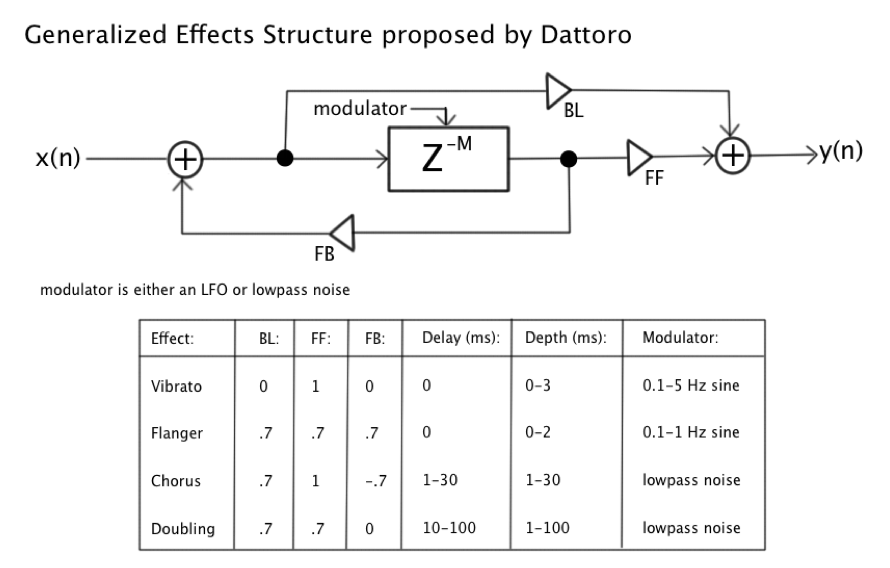
\includegraphics[width = 14cm]{generalizedEffect.png}
% 		\caption{generalized Effect structure}
% 		\label{fig:genEffect}
% 	\end{center}
% \end{figure}

% über name sprechen, sowohl spectrum als auch Impulsantwort(IIR variante) sind kammförmig. \\
% Eigentlich einfach ein delay, ein delay mit feedback im falle von IIR.\\




% \begin{figure}[h]
% 	\begin{center}
% 		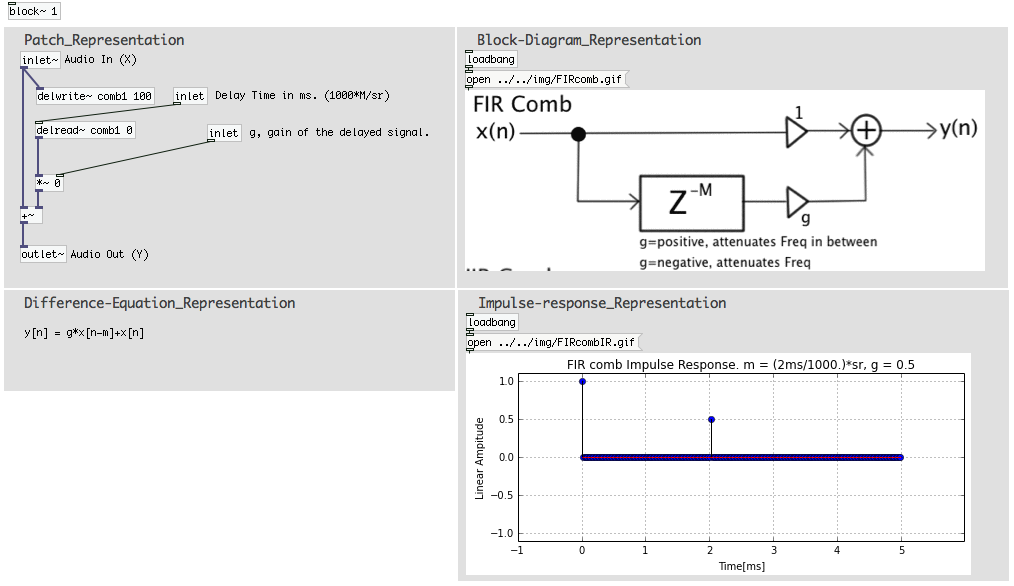
\includegraphics[width = 14cm]{img/combFIR_patch.png}
% 		\caption{Der Patch 01\_combFilter.pd}
% 		\label{fig:01_combFilter}
% 	\end{center}
% \end{figure}



% Zunächst nicht wichtig die versch. representationen zu verstehen. \\
% Patch representation kurz durchbesprechen. Sollte verständlich sein.\\

% Unterschiedliche representationen durchbesprechen.
% Fragen, abstimmen?, was die studenten für die angenehmste representation halten.



% \begin{itemize}
% 	\item Patch: vorteile: interaktiv, allgemein, reinfolge der events nachvollziehbar. Nachteil: nicht sehr übersichtlich. Nicht sehr konzis, nicht kompakt.
% 	\item Block Diagramm: übersichtlich, allgemein. Reinfolge der events klar, pfeile! Fluss, richtung, eindeutig. Nachteile: Nicht kompakt.
% 	\item differenzen gleichung: Vorteil: kompakt, konzis. Nachteil: reinfolge der events nicht klar ersichtlich: kein rezept, eher eine beschreibung. (nicht imperativ sondern deklarativ, va. im Fall von Feedback)
% 	\item Impulsantwort: \textbf{Frage: was ist ein Impuls?}  Vor/Nachteil: Nicht allgemein, nur ein spezieller zustand des systems beschrieben. Nicht kompakt, aber kann sehr intuitiv sein. Beispiele an tafel: IR von bypass-system, IR mit viel hall, IR von bandpass filter mit hoher resonanz, eventuell: differentiator, accumulator.
% 	\item andere representationen: text-code, transfer funktion, frequency response(magnitude + phase response/group delay)
% \end{itemize}




% \newpage


% \section {Moving Average}

% \textbf{Wo hat der kammfilter immer sein erstes Tal im spectrum?}
% Sinus an tafel malen.
% Antwort:
% bei 

% \(\lambda =  (2* \Delta t) \)
% (wobei \(\Delta t\) die delay zweit in sekunden. und \(\lambda\)  die periodendauer der gesuchten frequenz.) Daher:\\
% \(
% f_c = 1/(2* \Delta t)
% \)

% Nun wird das delay auf ein sample reduziert. Ein lowpass entsteht der seine grenzfrequenz bei sr/2 hat.\\

% Frage: was macht ein lowpass filter in der timedomain?


% \begin{figure}[h]
% 	\begin{center}
% 		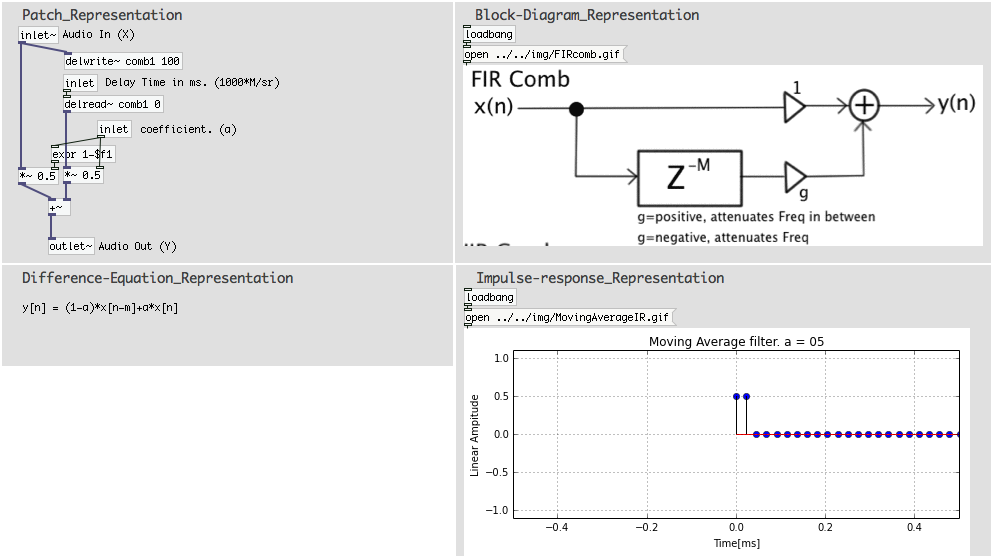
\includegraphics[width = 14cm]{movingAverage.png}
% 		\caption{movingAverage}
% 		\label{fig:movingAverage}
% 	\end{center}
% \end{figure}


% \textbf{EXKURS: VIDEO FILTER, lowpass, time domain erkennen.}


% \newpage
% \textbf{Frage:} Vergleiche original und die gefilterte variante (01.mov) . Was für ein filter könnte angewandt worden sein:
% \begin{enumerate}
%  	\item lowpass
%  	\item bandpass
%  	\item hipass
%  	\item notch
%  	\item nichts von alledem
%  \end{enumerate} 


% wie könnte ein highpass realisiert werden? Wie schaut der effekt eines highpass filters in der frequenz- und wie in der timedomain aus?


% \section{convolution, Faltung}

% Video (unten) zeigen, vorher erklären: \\

% conv theorem.

% http://youtu.be/\_vyke3vF4Nk?t=25m16s \\
% start bei min 25.

% \textbf{maxpatch}




% %%--------------------------------------------------------------------------
% %% IIR/FIR
% %%--------------------------------------------------------------------------
% \section {IIR/FIR}

% Je steiler die Filterflanke sein, je komplexer der filter sein soll, desto mehr delays werden benötigt.\\

% Wieso: einfache Erklärung: Um aus einem signal, das alle frequenzen enthält (zB dirac impuls) ein signal zu machen, das hauptsächlich sehr tiefe frequenzen enthält wird ein system benötigt das \glqq{}lange wellen\grqq{} zu produzieren im stande ist. 

% An tafel zeichnen: dirac impuls und unit step/ DC. Frage nach spectrum.\\

% frage nach FIR der diesen IR haben könnte.

% \textbf{Patch: lomgSimpleFir}

% Grenzfall: integrator macht aus unit impulse, \(delta [n]\), unit step signal\(u[n]\)(DC).

% Integrator an tafel malen.\\

% Daher:
% Es kann gezeigt werden dass ein feedback pfad einer unendlichen menge an delays gleichkommt, siehe IR.

% \textbf{Patch: 02\_combFilterIIR}

% nebenbei:
% linear phase = symmetrischer IR, immer FIR, daher weniger performant.
% Linear phase filter sind notwendig wenn die timedomain wellenform möglichst unbeeinträchtigt bleiben soll.

% \subsection{Onepole} % (fold)
% \label{ssub:onepole}

% % subsubsection subsubsection_name (end)
% onepole an tafel beschreiben. Block diagramm, malen, nach differenzengleichung fragen. Patch herzeigen.\\

% \textbf{patch: IIRtest} \\
% danach:\\
% \textbf{patch: IIRtest2} \\

% Fragwürdig aber falls interesse:
% onepole coeff berechnung zB:\\

% \begin{equation}
% a_0 = \frac{2 \pi f_c} {sr}
% \end{equation}

% oder

% \begin{equation}
% a_0 = sin(\frac{2 \pi f_c} {sr})
% \end{equation}


% \section{Hausübung}

% hausübung: Baue einen einen chorus. TESTSIGNAL AUSBESSERN! nicht noise!!

